\documentclass{exmppr}
\usepackage{tasks}
\usepackage{tikz}
\usepackage{epigraph}
\usepackage{verbatim}
\usetikzlibrary{arrows,shapes}
\usepackage{enumerate}

\institutename{Sardar Vallabhbhai National Institute of Technology, Surat}
\sem{1}%which semester
\coursename{Advanced Database Management System}%name of course
\ccode{CO619}%course code
\type{MidSem}%endsem or midsemm
\season{Summer}%winter, fall, summer, etc.
\batch{2018-19}% batch 2013-14,2014-15,2015-16 etc

\profname{Dipti P Rana}%name of prof

\newtheorem{exercise}{\bfseries}

\begin{document}
\begin{enumerate}

\item \begin{enumerate}
\item Explain the significant features of two educational institute applications which require support of non RDBMS.
\item Enlist the files to manage the physical database structure and explain the one file that is used to specify the physical structure of the database.
\item Enlist design principles to consider when developing query language for object management.
\item Enlist the properties used to preserve the integrity of the database system and explain any one of them.\\
{\centering OR}\\
Enlist the steps performed by database management system software if the transaction is committed.
\end{enumerate}
\item A company is managing employee information like id, name, work address, home address, contact numbers and dependent members. Each employee has two contact numbers primary and secondary. Write OQLs:
\begin{enumerate} 
\item Create the required objects and related tables.
\item Display all contact numbers of all employee with the ordering information of primary as `1' and secondary as `2'. Mention result type of your query.
\item Display all employees whose work address city is `Surat' and home address city is undefined. Mention result type of query.
\end{enumerate}
\item \begin{enumerate}
\item List major objectives of Distributed Database Management System.
\item List Types of Data replication and explain in brief.
\item Explain in brief strengths and weaknesses of Graph Database. Enlist any five typical use cases for Graph Databases.
\end{enumerate}

\item For the given scenario, write with reasons, which centrality measure is the most appropriate. And also rank the node/nodes according to the justified centrality measures.\\
\centering
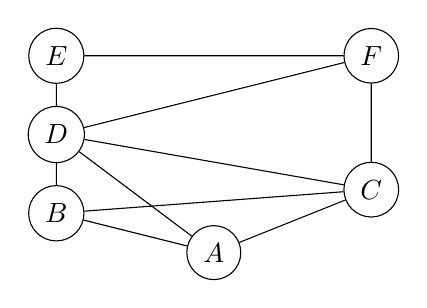
\begin{tikzpicture}[scale=1]
\node at (0,-.5) [circle,draw] (a) {$A$};
\node at (-2,0) [circle,draw] (b) {$B$};
\node at (2,.3) [circle,draw] (c) {$C$};
\node at (-2,1) [circle,draw] (d) {$D$};
\node at (-2,2) [circle,draw] (e) {$E$};
\node at (2,2) [circle,draw] (f) {$F$};

\draw (a) -- (b) -- (d) -- (e) -- (f) -- (c) -- (a) -- (d) -- (f);
\draw (b) -- (c) -- (d);
\end{tikzpicture}

\begin{enumerate}
\item Suppose the above \textbf{undirected} network refers to friendship network. Each node represents a person, and each represents friendship between the persons at ends. If you are interested in finding \textbf{the most popular person} in the network.
\item Suppose the above \textbf{undirected} network refers to information flow network of an organization. If you are interested in finding \textbf{the section that can most frequently control information flow in the network}.
\end{enumerate}
\end{enumerate}


\newpage
\begin{center}\section*{Answers}\end{center}
%\input{sol1.tex}

\end{document}
